\chapter{Methodology}
\label{chapt:methodology}

This chapter is devoted to a brief overview of our methods, namely the software tools that we use, and our approaches to modelling useful computations as dynamical systems.
Additional details are the focus of later chapters.

\section{Software}
\label{sec:software}

The simulations in this thesis make extensive use of the following Python software packages (versions listed when important):
\begin{itemize}
\item Nengo 2.8.0~\citep{bekolay2014}; to construct and simulate NEF models on the CPU, which depends on NumPy for its algebraic routines,
\item Nengo-Loihi 0.5.0~\citep{blouw2018a, nengoloihi}; to compile Nengo models onto the Loihi emulator and hardware (courtesy of ABR),
\item Nengo-Brainstorm~\citep[pre-release;][]{neckar2018optimizing, braindrop2019}; to compile Nengo models onto Braindrop (courtesy of Terry Stewart), which depends on PyStorm (courtesy of Femtosense),
\item HyperOpt 0.0.2~\citep{bergstra2015hyperopt}; to optimize the hyperparameters associated with RC networks,
\item Keras 2.2.4~\citep{gulli2017deep}; to train LSTMs and some custom RNNs,
\item TensorFlow 1.12.0~\citep{abadi2016tensorflow}; as a backend for Keras,
\item Seaborn~\citep{michael_waskom_2015_19108}; to generate figures, which depends on Matplotlib and Pandas for plotting and formatting data, respectively.
\end{itemize}
We do not take credit for any of the above software.
However, we have created the Python package, NengoLib 0.4.3~\citep[][patent~pending]{dynamicspatent, nengolib}, open-sourced on GitHub, to make the contributions of this thesis publicly available.
% which also depends on SciPy for many routines ported from MatLab
Code, \LaTeX{}, and instructions for reproducing figures, are located at: \url{https://github.com/arvoelke/phd/}.
Unless stated otherwise, all simulations use a time-step of $\dt{} = 1$\,ms, and assume the input signal is held constant across each time-step, also known as the ``zero-order hold''~(ZOH) assumption.
Experiments that implement the methods of \citet{boerlin2013predictive} in Nengo are currently unpublished (provided by Dan Rasmussen).

%\subsection{NengoLib}
%\label{sec:nengolib}

NengoLib includes the core code for most of the extensions discussed in chapter~\ref{chapt:nef-extensions} and the networks discussed in chapter~\ref{chapt:delays}.
It has been used by publications including
\citet{knight2016}, \citet{voelker2016a}, \citet{voelker2017iscas}, \citet{voelker2017neuromorphic}, and \citet{voelker2018}.
In addition, we use it to construct RC, FORCE, full-FORCE, and Nengo networks---each in spiking and non-spiking mode, and in an analogous manner to one another---in order to facilitate meaningful comparisons between these architectures.
A core feature of this software is a toolkit for constructing and analyzing linear time-invariant systems, in a number of representations (state-space, transfer function, zero-pole-gain), while being compatible with the synapses of Nengo.
This unifies the language used to build, describe, and analyze LTI networks, synapses, and sub-threshold neural dynamics.
We now summarize some additional features of this software that are used throughout.

\subsubsection{State-space realizations}

This section has been adapted from \citet[][appendix~A.3]{voelker2018}.
The state-space model (equation~\ref{eq:lti}) is \emph{not} a unique description of the input-output behaviour of an LTI system.
In general, one may consider any invertible matrix $T$ with the same shape as $A$, and observe that the state-space model $(TAT^{-1}\text{,}\, TB\text{,}\, CT^{-1}\text{,}\, D)$ has the same transfer function as $(A\text{,}\, B\text{,}\, C\text{,}\, D)$.
Thus, the state-space model is only unique up to a change of basis.
However, in the NEF, the basis $T$ may be ``absorbed'' into the representation of $\V{x}(t)$ by using the encoders $ET$ in Principle~1, which, in turn, results in the decoders $D^\V{f} \transpose{\left(T^{-1}\right)}$ from Principle~2.
In other words, considering an alternative state-space model is equivalent to considering a change of basis for the representation.
Nevertheless, in practice, when aiming to accurately represent $\V{x}(t)$ using few neurons, it is important to balance the relative range of values within each dimension, such that a typical trajectory for $\V{x}(t)$ stays within the space represented by the distribution of encoders, consistent with the samples of $S$ (see equation~\ref{eq:decoder_solution}), and the dynamic range of each neuron.

For this, there is a feature to \emph{balance} the range of values by numerically computing the $T$ that results in a ``balanced realization'' of $(A\text{,}\, B\text{,}\, C\text{,}\, D)$~\citep{laub1987computation, perevapproximation}.
We then set the encoders to be unit-length and axis-aligned, and optimize each dimension independently by using the methods from section~\ref{sec:principle2}.
There is also the support to normalize each dimension by a diagonal transformation $T$ with the $i^{\text{th}}$ diagonal equaling $\max_t \left| x_i(t) \right|^{-1}$ where $x_i(t)$ is obtained by simulating the ideal system directly on a randomly sampled input.
Finally, NengoLib supports a diagonal transformation $T$ with the $i^{\text{th}}$ diagonal corresponding to the reciprocal of two times the sum of the Hankel singular values~\citep{glover1987bounds} of the subsystem corresponding to $x_i(t)$.
This has the effect of bounding the absolute value of each dimension above by $1$ in the worst case~\citep{khaisongkram2007computing}.

In general, we find that each of the above methods to normalize state-space models typically improves the robustness of our networks across a wide range of parameters, but one is never strictly better than all others in every situation.

% Likewise, any change of basis in the state-space model of $F^H$ does not impact the dynamics of $F^H(H(s)^{-1})$
% But there is really no reason to do that as far as I can tell.
%It is worth noting that the mappings from section~\ref{sec:extensions}---with the exception of equations~\ref{eq:lambert-delay} and~\ref{eq:general-linear-approx}---do not alter the representation of $\V{x}(t)$.
%Disregarding these exceptions, the same choice of basis is conveniently carried over to the implemented network.
%Yet, it is also the case that the dynamics of the system mapped by equation~\ref{eq:general-linear-approx} do not depend on the chosen state-space model.
%This fact is proven implicitly in the following appendix, by characterizing the dynamics in terms of $F(s)$ and $H(s)$ alone.

%\url{https://arvoelke.github.io/nengolib-docs/master/notebooks/research/geometric\_decoders.html}

\subsubsection{Random sampling}

Many common routines in Nengo employ the use of high-dimensional random sampling~\citep{voelker2017, gosmann2018}, in particular the uniform sampling of encoders $\V{e}_i$ from the surface of the hypersphere, and the uniform sampling of evaluation points from $S$ (typically the interior of the hyperball).

Considering the NEF's optimization problem from equation~\ref{eq:decoder_solution},
Monte Carlo~(MC) sampling $S$ introduces $\bigoh{ m^{-\frac{1}{2}} }$ error into the integral, where $m$ is the number of samples, but this can be improved to $\widetilde{\mathcal{O}} \left( m^{-1} \right)$---effectively squaring $m$---by the use of quasi-Monte Carlo methods~\citep{fang1994, knight2016}.
For this, NengoLib overloads Nengo's default versions of these distributions, with its own method of uniformly scattering the samples using quasi-MC sampling.
Specifically, we take a scattered sample from the hypercube, and then apply the inverse transform method with a spherical coordinate transform~\citep{fang1994} to map samples onto either the hyperball or hypersphere.
This supports the use of any number of quasi-MC methods for sampling from the cube, although we have implemented the most promising ones: Sobol sequence and $R_2$~\citep{Sobol1967, quasimc}.

We find that quasi-MC sampling the encoders also improves the representation at low numbers of neurons on average, by ensuring a better tiling or coverage of the encoded space.
For efficient coding in higher dimensions, methods of randomly sampling points from the Leech lattice---a 24-dimensional Lattice built from \numprint{196560} unit-length vectors, with beautiful mathematical properties regarding their similarity in relation to efficient sphere-packing and error-correction codes~\citep{Conway1999}---used by \citet{knight2016} are also available in software.

% \subsubsection{Vector Oja Learning Rule}

\section{Dynamics as a language}
\label{sec:dynamics-language}

As discussed in section~\ref{sec:nef-turing}, dynamical systems represent a complete (i.e.,~universal) model of computation.
But how are useful high-level computations embedded into such systems?
To this end, we are interested in developing a language for describing useful algorithms within the dynamical modelling framework of the NEF, and libraries for combining these models within Nengo.

Early work by \citet{eliasmith2003a} has shown that many important neurobiological systems, such as the nuclei involved in horizontal eye control, may be modelled as an integrator.
That is, some velocity signal, indicating a desired direction, is represented by one population and then integrated by another.
Such systems are describable as a one-dimensional linear time-invariant system (see equation~\ref{eq:lti}), such as the one demonstrated in section~\ref{sec:chaos} using ten spiking neurons. 
When extended to higher dimensions, this same system is capable of storing multiple items in series, and has consequently been applied to build sophisticated models of working memory~\citep{singh2004, choo2010}.

Oscillatory dynamics (e.g.,~relaxation oscillators), such as those modelled in \citet{eliasmith2000b} have utility in generating rhythmic activity to support various computations.
For example, theta oscillations in the range of $4$--$12$\,Hz, through a phenomenon known as phase precession, have been shown to support the encoding of spatial information using Nengo~\citep{o1993phase, orchard2013does}.
Likewise, a bank of oscillators can be used to facilitate motion processing in the early visual system~\citep{huzook2012}. 

Attractor networks describe a much broader class of nonlinear dynamical systems that capture many important phenomena observed in neurobiological systems~\citep{amit1989modeling, eliasmith2005b}.
When oscillations, integrators, and point attractors, are all combined, networks may generate complex trajectories through space~\citep{ijspeert2013dynamical, dewolf2017}.
By arranging all of these building blocks in an engineered fashion, together with feed-forward (i.e.,~synaptic) dynamics coupling various modules, complex systems such as Spaun may carry out end-to-end cognitive tasks and even learn to follow general sets of instructions~\citep{eliasmith2012, choo2018}.
The role of chapter~\ref{chapt:delays} is to unveil another class of dynamical systems for continuous nonlinear memory, that connects with ``time cell'' data from the neuroscience literature, and naturally fits into this framework.
But first, we describe a few concrete examples to help illustrate the universality of dynamical descriptions of computation, in a number of distinct contexts.

\subsection{Winner-take-all}

Winner-take-all~(WTA) circuits essentially engineer a ``$\max$'' function that pools across \emph{spatial} dimensions.
These systems may be described in state-space using nonlinear differential equations, that compete with one another in order to resolve the correct solution over time, as in an attractor network~\citep{usher2001time, gosmann2017a}.
Here, we are interested in a very different kind of WTA circuit that must compute its $\max$ across temporal dimensions.
We call this circuit a ``peak detector''.\footnote{%
This problem was proposed by Jan Gosmann (unpublished).}
Specifically, we suppose the input vector, $\V{u} \in \mathbb{R}^m$, is supplied online, one dimension at a time, such that:
$$\V{u}[k] = \transpose{\left( u[k] \text{,}\, u[k-1] \text{,}\, \ldots \text{,}\, u[k-m] \right)}$$
for some (possibly infinite) number of samples, $m \ge 1$.
In this context, determining the maximum of $\V{u}[k]$ is equivalent to the task of tracking the peak of the past history of the discrete-time signal, $u[k]$ (see Figure~\ref{fig:wta-peak-detector}), at a sampling interval of $\dt{}$.
In other words, the problem of tracking the maximum across time, is equivalent to a WTA mechanism where the input dimensions are provided sequentially, as opposed to being provided all at the same moment in time (as is usually the case).

\begin{figure}
\centering
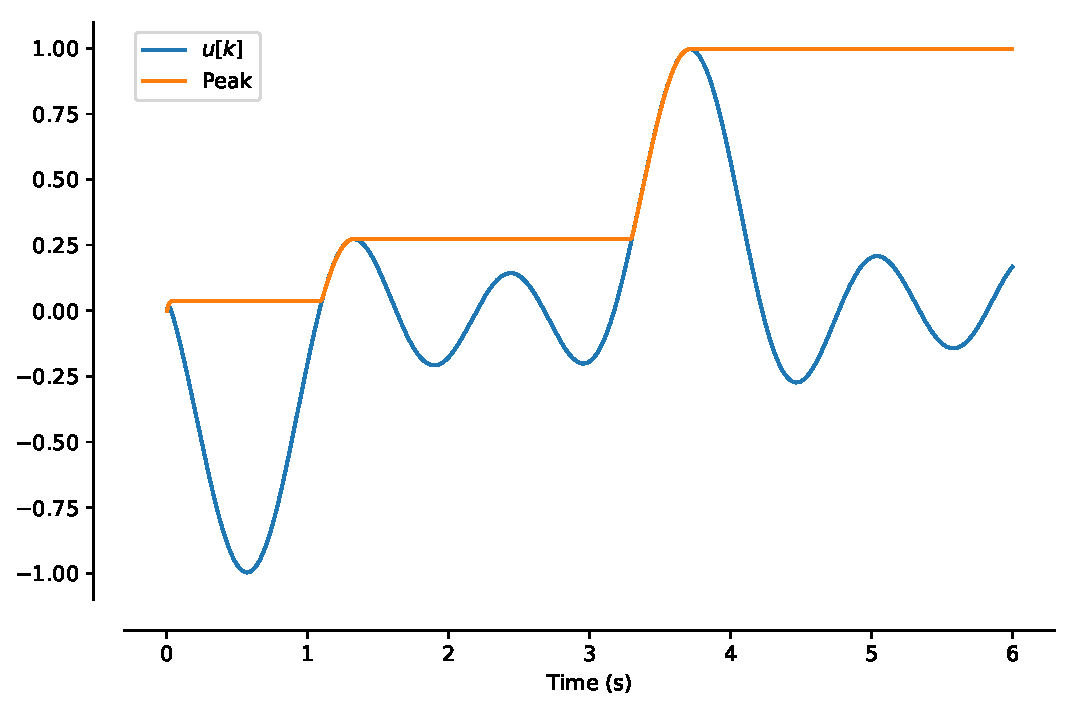
\includegraphics[width=0.5\textwidth]{wta-peak-detector}
\caption{ \label{fig:wta-peak-detector}
  An ideal ``peak detector'' implemented as a discrete-time dynamical system.
}
\end{figure}

In the limit of $\dt{} \rightarrow 0$, the desired continuous-time dynamical system is:
\begin{equation}
\label{eq:peak-detector-continuous}
\dot{x}(t) = f(x(t), u(t)), \quad f(x, u) = \kappa \left[u - x \right]_+
\end{equation}
where $\left[ \cdot \right]_+$ denotes positive half-wave rectification. $\kappa > 0$ is a time-constant that determines how quickly the state should adjust to the positive difference. Note that in a purely continuous-time system, assuming no noise, $\kappa$ can be made arbitrarily large, in order to track the peak arbitrary quickly. 
However, since we have a discrete sampling time, our desired dynamical system is:
\begin{equation}
\label{eq:peak-detector-discrete}
x[k + 1] = \bar{f}(x[k], u[k]), \quad \bar{f}(x, u) = \bar{\kappa} \left[u - x \right]_+ + x
\end{equation}
where $0 < \bar{\kappa} \le 1$ is a (dimensionless) discrete time-constant.
Equation~\ref{eq:peak-detector-discrete} is related to equation~\ref{eq:peak-detector-continuous} by $\bar{\kappa} = \left( \dt{} \right) \kappa$, assuming Euler integration.
Note that $\bar{\kappa} = 1$ will give a perfect peak detector, assuming no noise.

In Figure~\ref{fig:wta-peak-detector}, we implement a peak detector by using Nengo directly as a dynamical systems simulator. This does not use any neurons, but rather digitally implements equation~\ref{eq:peak-detector-discrete} with $\bar{\kappa} = 1$ by coupling each variable in the correct way:
\begin{python}
with nengo.Network() as model:
    u = nengo.Node(stim)  # stim defines the test input signal
    peak = nengo.Ensemble(1, dimensions=2, neuron_type=nengo.Direct())
    nengo.Connection(u, peak[1], synapse=None)
    function = lambda x: (x[1] - x[0]).clip(min=0) + x[0]
    nengo.Connection(peak, peak[0], synapse=~z, function=function)
\end{python}
We remark that $\textasciitilde z$ is a dynamical primitive in NengoLib that implements a single time-step delay, in correspondance with the $\mathcal{Z}$-transform in signal processing.
This illustrates the utility of discrete-time dynamical systems, the flexibility of this framework for describing useful computations, and the versatility of Nengo as a programming tool for simulating such systems.
Both continuous-time and discrete-time versions of this system may be implemented using spiking neurons as well (not shown).
In chapter~\ref{chapt:nef-extensions} we will address the implementation of such systems using neural populations in both analog and digital hardware.

\subsection{Unsupervised learning}
\label{sec:unsupervised}

This section has been adapted from \citet{voelker2014a}, and discusses the dynamics of an unsupervised learning rule used by \citet{voelker2014controlling}, \citet{trujillo2014a}, and \citet{aubin2016a}.
This has been implemented on SpiNNaker~\citep{knight2016}, and is discussed in some detail by \citet{aubin2018}.
Here we expose the dynamics of this learning rule, while highlighting its function for sparsifying across space in large-scale models.

Associative memories have been an active area of research over the last forty years~\citep{willshaw1969nonholographic, kohonen1972, hopfield1982} because they form a central component of many cognitive architectures~\citep{Pollack1988, Anderson1998}.
We focus specifically on associative memories that store associations between arbitrary pairs of neural states.
When a noisy version of an input state vector is presented to the network, it must output a ``clean'' version of the associated state vector.
\citet{stewart2011biologically} has built such a memory network, possessing a number of desirable properties including: high accuracy, a fast, feed-forward recall process, and efficient scaling, requiring a number of neurons linear in the number of stored associations.
 These memories have played a central role in several cognitive models including Spaun, as well a proposal for human-scale, biologically-plausible knowledge representation~\citep{crawford2015}.
However, these memories are constructed using an offline optimization method that is not biologically-plausible.

We describe a method for building large-scale networks for online learning of associations using spiking neurons.
Connection weights can be arrived at through a biologically-plausible, online learning process featuring a novel synaptic learning rule inspired in part by the well-known Oja learning rule~\citep{oja1989neural}.
We call this rule the \emph{voja} learning rule (for ``vector Oja'').
Although the network itself is feed-forward, the dynamics that carry out the important computations are embedded within the learning rules that modify its synaptic weights online.
We now describe the learning rule.

Given a learning rate $\eta$, an input vector $\V{x}$ encoded by the activity of the input layer, the filtered activity $a(t)$ of  neurons in the middle layer, and the matrix $E$ whose rows are the ``preferred direction'' vectors of the middle layer neurons, we modify the preferred direction vectors of the middle layer neurons according to the equation:
\begin{align} \label{voja}
    \Delta{E} = \eta \left( a(t) \transpose{\V{x}} - a(t)E \right) = \eta a(t) \left( \begin{pmatrix} \transpose{\V{x}} \\ \vdots \\ \transpose{\V{x}} \end{pmatrix} - E \right) \text{.}
\end{align}
To understand the effect of this rule over time, we set $\Delta{E_i} = 0$ and solve for the fixed point.
This gives $a_i(t) \V{x} = a_i(t) \V{e}_i$, and thus, for a particular $\V{x}$, convergence is characterized by:
\begin{align} \label{stability}
    [\Delta{\V{e}_i} = 0]  \iff  [a_i(t) > 0  \implies  \V{e}_i = \V{x}] \text{.}
\end{align}
In plain words, the encoding vectors of the neurons that become active will, over time, become more active and store the input within its encoder.
The effect of this rule is to make a sparse subset of the neurons fire only when $\V{x}$ or a similar enough (i.e.,~noisy) version of it, is presented (see Figures~\ref{fig:voja-spinnaker} and~\ref{fig:voja-encoders}).
The preferred direction vectors of each neuron are embedded within the synaptic weights projecting from the previous layer.
Thus, this can be realized as a local learning rule by multiplying the decoders through and expressing the update in its weight with the $j^\text{th}$ presynaptic neuron~\citep{knight2016}:
\begin{align}
  \label{eq:voja-weights}
  \Delta \omega_{ij} = \Delta \V{e}_i \cdot \V{d}_j = \eta \, a_i (\V{d}_j \cdot \V{x} - \omega_{ij}) \text{.}
\end{align}
In effect, this rule embeds some useful computation---the unsupervised learning of associations between inputs and outputs---as a localized dynamical system within the computation of individual synapses.
We demonstrate similar ideas in the following section, as they pertain to supervised learning and oscillations.

\begin{figure}
    \centering
  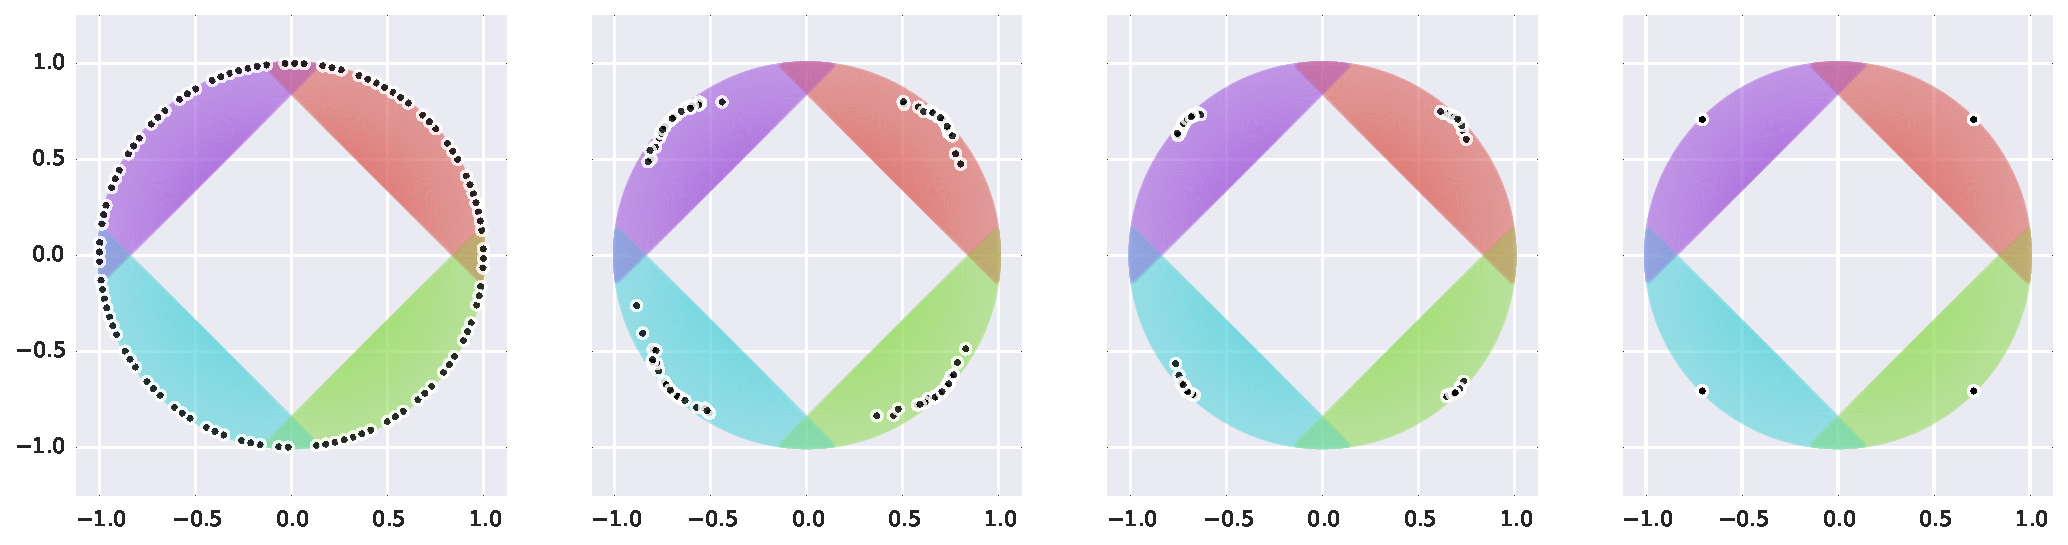
\includegraphics[width=\textwidth]{voja-spinnaker}
  \caption{
The effect of Voja on the encoders of a 2-dimensional population, over time.
Each point corresponds to the encoder of one of \num{100} neurons.
Four input vectors are chosen of the form $(\pm 1 / \sqrt{2}, \, \pm 1 / \sqrt{2})$, and their areas of attraction within the unit circle are indicated by shaded regions ($c = 0.6$).
As the simulation progresses, from left to right, each encoder converges to one of the possible inputs.
Reproduced from \citet{knight2016}.
  \label{fig:voja-spinnaker}
    }

  \vspace{1em}

    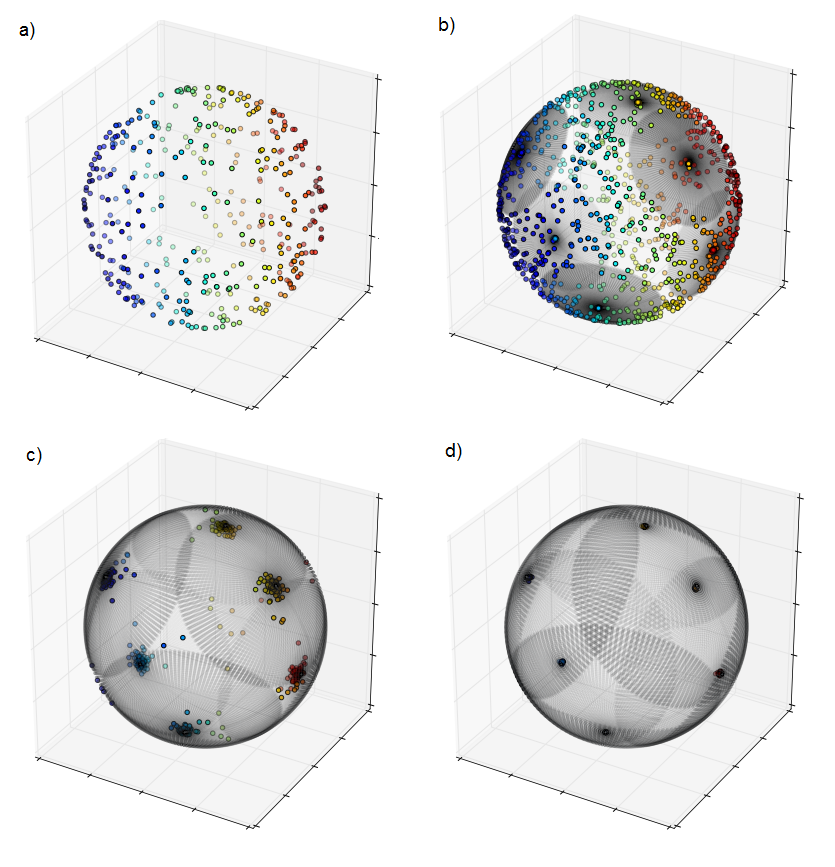
\includegraphics[width=0.5\textwidth]{voja-encoders}
    \caption{Input vector clustering of a 3-dimensional ensemble, presented with 6 evenly spaced $\V{x}$. (a) The initial clustering, before any input has been given. (b) Each input vector has been shown for two seconds of simulation time, with intercepts set to $cos \left(\frac{\pi}{6} \right)$. Gray plates show the area of attraction for each input vector. (c) Same as b, with intercepts chosen to give $p_i = 1/6$. (d) Same as b, with intercepts set to $cos \left(\frac{\pi}{3} \right)$. \label{e3d}
    Reproduced from \citet{voelker2014a}.
       \label{fig:voja-encoders}
    }
\end{figure}

\subsection{Supervised learning}

This section has been adapted from preliminary work by \citet{voelker2015} and \citet{voelker2017c}.
This approach highlights the utility in shifting perspectives in learning to that of a dynamical system embedded within some larger function.
In particular, online learning is nothing more than a dynamical system realized by localized computations within the network.
We illustrate this by unifying Nengo's supervised learning and the NEF's dynamical systems framework at a theoretical level, and leverage the resulting relationship in a practical spiking example with online learning.

The NEF typically learns its connection weights offline, but Nengo also supports a number of biologically-plausible supervised and unsupervised learning rules to learn these weights online~\citep{bekolay2011a}.
Prescribed Error Sensitivity~\citep[PES;][]{bekolay2013} is a biologically-plausible Hebbian supervised learning rule that is frequently used within Nengo models.
PES modifies the connection weights between populations of neurons to minimize an external (i.e.,~supervised) error signal.
It is equivalent in function to a single-layer application of gradient descent, applied online (i.e.,~stochastically) to its current input and supervised output.
This learning rule has been used to model episodic memory~\citep{trujillo2014}, hierarchical reinforcement learning~\citep{rasmussen2017}, adaptive motor control~\citep{komer2015, dewolf2016}, and many other tasks~\citep{aubin2018, choo2018}.
We note that the PES learning rule is also supported by Loihi~[personal communication].

We solve the discrete dynamical system for the case of constant inputs and no noise, to show that the decoding vectors given by the NEF have a simple closed-form expression in terms of the number of simulation timesteps. Moreover, with $\gamma = (1 - \kappa \|\V{a}\|^2) < 1$, where $\kappa$ is the learning rate and $\V{a}$ is the vector of firing rates, the error at timestep $k$ is the initial error times $\gamma^k$. Thus, $\gamma > - 1$ implies exponential convergence to a unique stable solution, $\gamma < 0 $ results in oscillatory weight changes, and $\gamma \le -1$ implies instability.
\begin{theorem}
\label{thm:pes-dynamics}
{\normalfont \citep{voelker2015}}
\newline
Let $\gamma = (1 - \kappa \|\V{a}\|^2) < 1$, and $e_0 = y^* - \V{d}[0]^T \V{a}$, then:
\begin{align}
\label{eq:dk}
\V{d}[k] &= \V{d}[0] + e_0\frac{\V{a}}{\|\V{a}\|^2} (1 - \gamma^k)\text{, \quad $k \in \mathbb{N}$} \text{,}
\end{align}
and so the error at timestep $k$ is $y^* - \V{d}[k]^T \V{a} = e_0\gamma^k$. In particular, if $\gamma > - 1$, then $\V{d}[\infty]$ exists and is given by the unique solution,
\begin{align}
\label{eq:dinf}
\V{d}[\infty] &= \V{d}[0] + e_0\frac{\V{a}}{\|\V{a}\|^2} .
\end{align}
On the other hand, if $\gamma \le -1$ then the system is unstable.
The proof is given by \citet{voelker2015}.
\end{theorem}

Continuing this work, we solve for the dynamics of PES, while filtering the error with an arbitrary linear synapse model. 
For the most common case of a lowpass filter, the continuous-time weight changes happen to be characterized by a second-order bandpass filter with frequency $\omega = \sqrt{\tau^{-1} \kappa \|\V{a}\|^2 }$ and bandwidth $Q = \sqrt{\tau \kappa \|\V{a}\|^2 }$, where $\tau$ is the exponential time constant, $\kappa$ is the learning rate, and $\V{a}$ is the activity vector.
Therefore, the error converges to zero, yet oscillates if and only if $\tau \kappa \|\V{a}\|^2 > 1/4$.
This provides a heuristic for setting $\kappa$ based on the synaptic $\tau$, and a method for engineering remarkably accurate decaying oscillators using only a single spiking leaky integrate-and-fire neuron.

Theorem~\ref{thm:pes-dynamics} fully characterized the discrete-time dynamics of PES under the restricted setting of a constant input signal, constant reference signal, and no noise.
Due to the absence of noise, no filter was required for the error signal.
However, for spiking networks considered in practice, a lowpass is applied to the error to filter out spike-noise~\citep[e.g.,][]{dewolf2016, rasmussen2017},  
We now relax the assumption of a constant reference signal, and apply an arbitrary linear filter to the error signal.
For simplicity, we do so for the case of a continuous-time simulation, but our analysis can also be applied to the discrete-time setting via the $\mathcal{Z}$-transform.
To keep our analysis tractable, we still assume a constant input signal, and briefly discuss implications for the general dynamic setting.

We begin by formulating a mathematical description of the network, present our theoretical results, prove them mathematically, validate them with numerical simulations, and demonstrate the utility of this analysis by engineering oscillators with predetermined frequencies and decay rates.
Finally, we conclude by discussing some implications for learning spiking dynamical networks online.

\subsubsection{Prescribed Error Sensitivity}

\begin{figure}
\centering
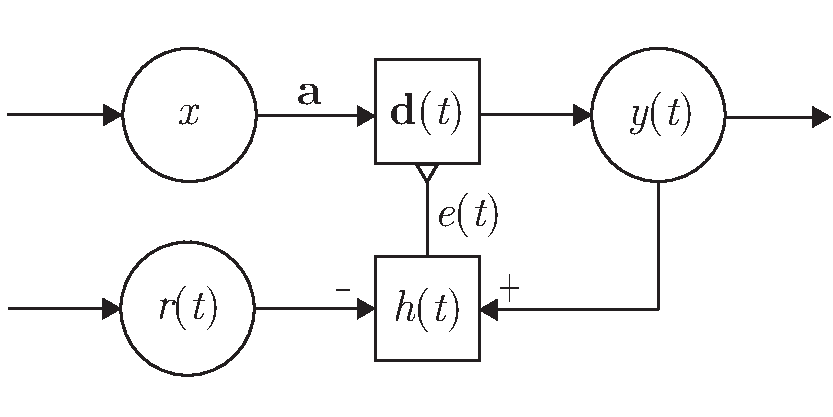
\includegraphics[width=0.5\textwidth]{pes-filtered-network}
\caption{\label{fig:pes-filtered-network}
  Network diagram used to analyze the PES rule.
  A constant input $x$ is represented by a population of $n$ spiking neurons with the activity vector $\V{a} \in \mathbb{R}^n$.
  A dynamic reference signal $r(t)$ determines the error $e(t) = \left((y - r) \ast h\right)(t)$~(equation~\ref{eq:error}), which in turn drives $y(t)$ towards $r(t)$ by modulating the connection weights via PES~(equation~\ref{eq:pes}).
  These learned connection weights decode $y(t)$ via the decoders $\V{d}(t) \in \mathbb{R}^n$~(equation~\ref{eq:decoding}).
  A linear filter $h(t)$ models the post-synaptic current induced by each spike.
  Reproduced from \citet[][Figure~1]{voelker2017c}.
}
\end{figure}

Consider a network in Nengo, containing a population of $n$ spiking neurons, encoding the constant scalar input $x$.
Let $\V{a} \in \mathbb{R}^n$ be the average (i.e.,~rate) activity of each neuron in response to this encoding.\footnote{Here on, we assume that $\V{a} \ne \V{0}$, otherwise PES will have no effect.}
This vector is determined by the first principle of the NEF, and remains fixed for constant $x$.
The \emph{decoders} $\V{d}(t) \in \mathbb{R}^n$ determine the scalar output $y(t)$ via the dot-product:
\begin{equation}
\label{eq:decoding}
y(t) = \transpose{\V{a}} \V{d}(t)  \text{.}
\end{equation}
The PES rule learns these decoders, online, according to the following dynamics:
\begin{equation}
\label{eq:pes}
\dot{\V{d}}(t) = -\kappa e(t) \V{a} \text{,}
\end{equation}
where $\kappa > 0$ is the learning rate,\footnote{$\kappa$ is automatically scaled by $n^{-1}$ in Nengo, to balance the linear scaling of $\|\V{a}\|^2$.} and $e(t)$ is the chosen error signal:\footnote{Signs are flipped in \citet{voelker2015}; equations~\ref{eq:pes} and~\ref{eq:error} are consistent with Nengo.}
\begin{equation}
\label{eq:error}
e(t) = \left((y - r) \ast h \right)(t) \text{,}
\end{equation}
where $r(t)$ is the reference (i.e.,~ideal) output, and $h(t)$ is some arbitrary linear filter modeling the post-synaptic current (PSC) induced by a spike arriving at the synaptic cleft.
Typically, $h(t)$ is a first-order lowpass filter with time constant~$\tau > 0$ (i.e.,~equation~\ref{eq:lowpass-laplace}):
\begin{equation}
\label{eq:lowpass}
h(t) = \frac{1}{\tau} e^{-\frac{t}{\tau}} \iff H(s) = \frac{1}{\tau s + 1} \text{.}
\end{equation}
%Thus, the connection weights learn to represent $r$ when presented with $x$.
The final network is summarized in Figure~\ref{fig:pes-filtered-network}.
This also naturally extends to the case where $x$ and $y$ are vectors (using a population code), but we consider the scalar case for simplicity. 

Now, we aim to characterize the dynamics of $e(t)$ in response to the control signal $r(t)$.
Alternatively, we could characterize the dynamics of $y(t)$ or $\V{d}(t)$, but the former is easier to work with, while describing the latter via equations~\ref{eq:decoding} and~\ref{eq:pes} (i.e.,~by integrating $e(t)$).

\begin{theorem}
\label{thm:pes-filtered}
{\normalfont \citep{voelker2017c}}
\newline
Let $\phi = \tau \kappa \|\V{a}\|^2$.
For the network described in Figure~\ref{fig:pes-filtered-network}, we have:
\begin{equation}
\label{eq:time-domain}
e(t) = (r \ast f)(t) \text{,}
\end{equation}
where: %\footnote{$\mathcal{L}^{-1} \left\{ \cdot \right\}$ denotes the inverse Laplace transform.}
\begin{equation}
\label{eq:s-domain}
F(s) = \frac{-s}{s H(s)^{-1} + \kappa \|\V{a}\|^2} \text{,} 
%f(t) &= \mathcal{L}^{-1} \left\{ F(s) \right\} \\
%H(s) &= \mathcal{L} \left\{ H(t) \right\} \text{.}
\end{equation}
hence $F(s)$ is the transfer function from $R(s)$ to $E(s)$.
For the case of a first-order lowpass filter (equation~\ref{eq:lowpass}),
\begin{align}
\label{eq:lowpass-solution}
\implies \quad F(s) = \frac{-s}{\tau s^2 + s + \kappa \|\V{a}\|^2} &= \frac{-\left( \kappa \|\V{a}\|^2 \right)^{-1} s}{\left(\frac{1}{\omega^2}\right)s^2 + \left(\frac{1}{\omega Q}\right) s + 1} \quad\quad \\
\omega &= \sqrt{\tau^{-1} \kappa \|\V{a}\|^2 } \label{eq:bandpass-w} = \tau^{-1} \sqrt{\phi} \\
Q &= \sqrt{\tau \kappa \|\V{a}\|^2 } = \sqrt{\phi} \label{eq:bandpass-Q} \text{.}
\end{align}
Thus, $F(s)$ is a second-order $Q$-bandpass filter with frequency $\omega$ in radians per second ($\frac{\omega}{2 \pi}$ is the frequency in hertz)~\citep[][pp.~8.9--8.10]{zumbahlen2011linear}.
The poles of $F(s)$ are:
\begin{equation}
\label{eq:poles}
s = \frac{-1 \pm \sqrt{1 - 4 \phi}}{2\tau} \text{.}
\end{equation}
%with complex magnitude $|s| = \omega$.
Since $\phi > 0$, this system is exponentially stable, and, moreover, the impulse response, $f(t)$, is a decaying oscillator if and only if $\phi > 1/4$.
\end{theorem}

\begin{proof}
We begin by transforming equations~\ref{eq:decoding}--\ref{eq:error} into the Laplace domain:
\begin{align*}
Y(s) &= \transpose{\V{a}} \V{D}(s) \\
s\V{D}(s) &= - \kappa E(s) \V{a} \\
E(s) &= \left(Y(s) - R(s) \right) H(s) \text{.\footnotemark}
\end{align*}
\footnotetext{This has nice form since $\V{a}$ is a constant -- otherwise multiplication of two time-varying signals becomes a complex integral in the Laplace domain.}%
Substituting the first two equations into the last, yields:
\begin{align*}
&& E(s) &= \left( \transpose{\V{a}} \V{D}(s) - R(s) \right) H(s) \\
&& &= \left( - \transpose{\V{a}} s^{-1} \kappa E(s) \V{a} - R(s) \right) H(s) \\
&& &= - \kappa \|\V{a}\|^2 s^{-1} H(s) E(s) - R(s) H(s) \\
\iff && \left(1 + \kappa \|\V{a}\|^2 s^{-1} H(s) \right) E(s) &= - R(s) H(s) \\
\iff && E(s) &= R(s) \left( \frac{-H(s)}{1 + \kappa \|\V{a}\|^2 s^{-1} H(s)} \right) \\
&& &= R(s) \left( \frac{- s}{s H(s)^{-1} + \kappa \|\V{a}\|^2} \right) \\
&& &= R(s) F(s) \text{.} % \tag*{\qed}
\end{align*}

Equations~\ref{eq:time-domain} and~\ref{eq:s-domain} follow from the convolution theorem.
Equations~\ref{eq:lowpass-solution}--\ref{eq:bandpass-Q} are verified by substituting $H(s)^{-1} = \tau s + 1$ into equation~\ref{eq:s-domain}.

The poles of the system (equation~\ref{eq:poles}) are obtained by applying the quadratic formula to the denominator polynomial from equation~\ref{eq:lowpass-solution} ($\tau s^2 + s + \kappa \|\V{a}\|^2$).
%The magnitude of the poles ($\omega$) come from the polar coordinate solution to this quadratic.
Exponential stability is implied by both poles being strictly in the left half-plane.
Lastly, $f(t)$ oscillates if and only if the poles are complex, if and only if the discriminant ($1 - 4 \phi$) is negative, if and only if $\phi > 1 / 4$.
\end{proof}

%As a corollary to equation~\ref{eq:lowpass-solution} and the Laplace transform of equations~\ref{eq:decoding} and~\ref{eq:pes},
%\begin{equation}
%y(t) = (r \ast g)(t) \text{,}
%\end{equation}
%where:
%\begin{equation}
%G(s) = \frac{\kappa \|a\|^2}{\tau s^2 + s + %\kappa \|\V{a}\|^2} \text{,}
%\end{equation}
%which has the same dynamics as equation~\ref{eq:lowpass-solution} with a phase shift.
%But these are (unfiltered) spikes...

\subsubsection{Validation}

We construct the network from Figure~\ref{fig:pes-filtered-network} using Nengo, with only $n = 1$ spiking leaky integrate-and-fire neuron (mean firing rate of $262\,$Hz),\footnote{%
Spikes are used in place of $\V{a}$ in equations~\ref{eq:decoding} and~\ref{eq:pes}.} $\tau = 0.1\,$s (equation~\ref{eq:lowpass}), $x = 0$, and $\kappa$ such that $\phi > 1/4$.
We construct the transfer function from equation~\ref{eq:lowpass-solution} using NengoLib:
\begin{python}
import nengolib
from nengolib.signal import s
H = nengolib.Lowpass(tau)
F = -s / (s/H + kappa*a.dot(a))
\end{python}
where \texttt{tau}~$\leftarrow \tau$ is the time constant of the synapse, \texttt{kappa}~$\leftarrow \kappa$ is the learning-rate supplied to Nengo (divided by $n$), and \texttt{a}~$\leftarrow \V{a}$ is the NumPy array for the population's activity.
We evaluate $(r \ast f)(t)$ using \texttt{F.filt(r, dt=dt)}, and compare this to the $e(t)$ obtained numerically in simulation.
The \texttt{filt} method automatically discretizes $F(s)$ according to the simulation time-step (\texttt{dt}~$= 1\,$ms) using zero-order hold (ZOH).\footnote{Technically, for a discrete-time simulation, the problem and results should have been formulated in the discrete-time domain using the $Z$-transform to begin with, as opposed to discretizing at the end, but the difference is quite subtle.}

In Figure~\ref{fig:pes-error}, we confirm that $(r \ast f)(t)$ approximates the numerical $e(t)$ given white noise $r(t)$.
In Figure~\ref{fig:pes-oscillator}(Top), we exploit our knowledge of the impulse response, $f(t)$, to engineer a number of decaying oscillators by controlling $r(t)$.
In Figure~\ref{fig:pes-oscillator}(Bottom), we evaluate \texttt{np.abs(F.evaluate(freqs))} at a variety of frequencies (\texttt{freqs}) to visualize the bandpass behaviour of each filter.

\begin{figure}
\centering
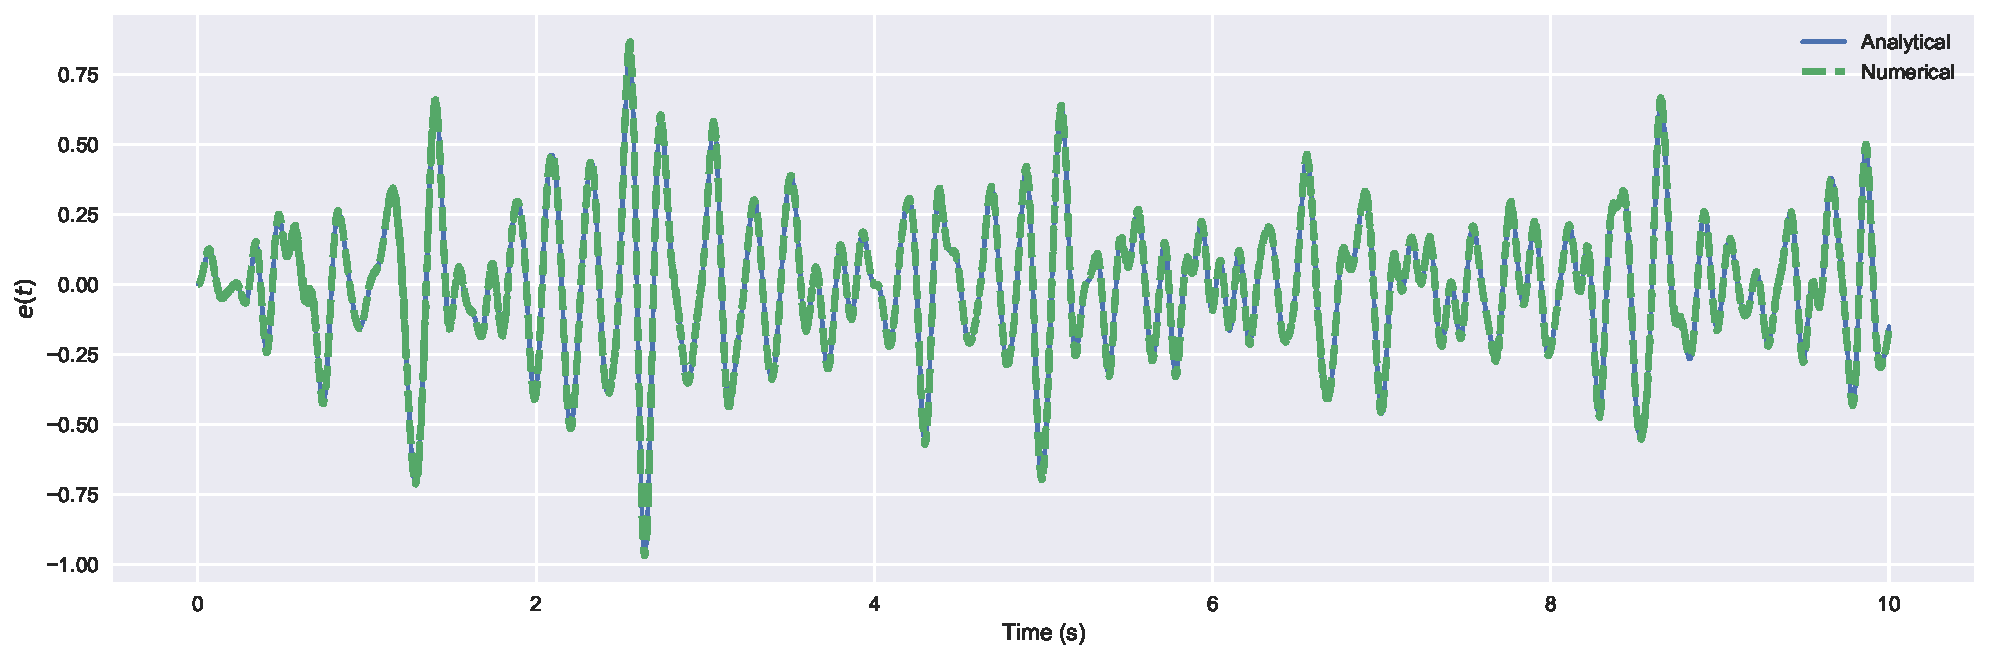
\includegraphics[width=1.0\textwidth]{pes-error}
\caption{ \label{fig:pes-error}
  Comparison of the analytical error (equation~\ref{eq:lowpass-solution}) to the numerical $e(t)$ obtained by simulating the network from Figure~\ref{fig:pes-filtered-network} ($\kappa = \numprint{e-3}$).
  The control signal $r(t)$ is randomly sampled white noise with a cutoff frequency of $10\,$Hz.
  The normalized root-mean-square error is approximately $3.7\%$.
  Reproduced from \citet[][Figure~2]{voelker2017c}.
}
\end{figure}

\begin{figure}
\centering
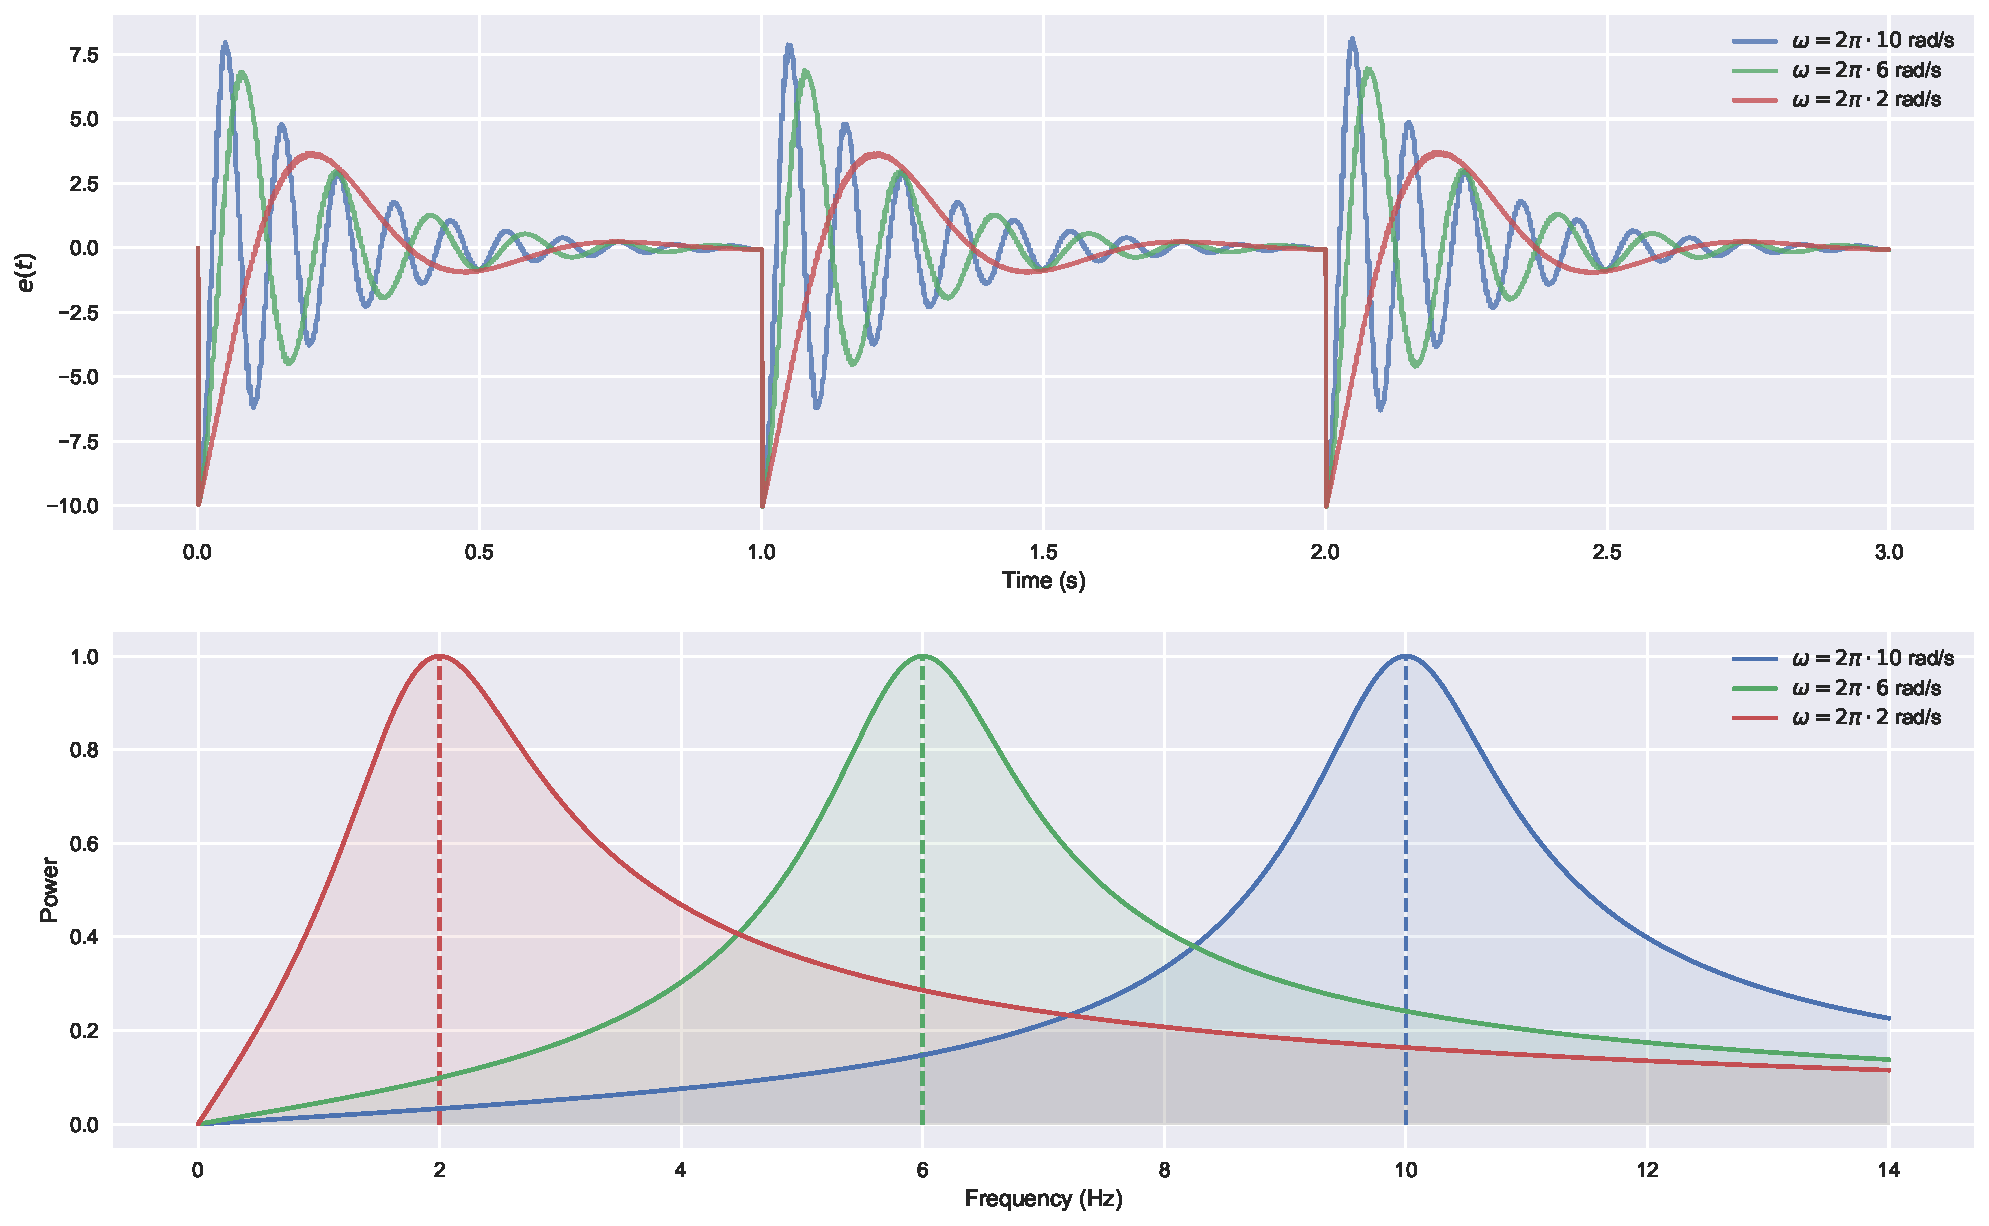
\includegraphics[width=1.0\textwidth]{pes-oscillator}
\caption{ \label{fig:pes-oscillator}
  Harnessing the dynamics of PES with various $\kappa$ to engineer decaying oscillators with predetermined frequencies ($\omega$) and bandwidths ($Q$), using only a single leaky integrate-and-fire neuron.
  The time constant of the first-order lowpass filter is fixed at $\tau = 0.1\,$s, while $\kappa$ is set to achieve the desired $\omega$ via equation~\ref{eq:bandpass-w}.
  (Top)~Once every second, $r(t)$ is set to a unit-area impulse.
  Consequently, $e(t)$ oscillates according to the impulse response, $f(t)$.
  (Bottom)~Visualizing the ideal frequency response of $F(s)$ (equation~\ref{eq:lowpass-solution}).
  Dashed lines at $\omega$ (equation~\ref{eq:bandpass-w}) align with the peak of each bandpass filter, or equivalently the frequency of each oscillation.
  The width of each filter is proportional to the decay rate $Q^{-1}$ (equation~\ref{eq:bandpass-Q}).
  Reproduced from \citet[][Figure~3]{voelker2017c}.
}
\end{figure}

\subsubsection{Discussion}

Since $\phi = \tau \kappa \|\V{a}\|^2 > 1/4$ if and only if the weights oscillate, this motivates a simple heuristic for setting the learning rate to prevent oscillatory weight changes: set $\kappa \le \frac{1}{4 \tau \|\V{a}\|^2}$, where $\|\V{a}\|^2$ is maximal over all possible activity vectors.
In this case, equation~\ref{eq:lowpass-solution} factors into a (differentiated) double-exponential:
\begin{equation*}
F(s) = \frac{-\tau_1 \tau_2 s}{\tau (\tau_1 s + 1)(\tau_2 s + 1)} = \left( - \tau_1 \tau_2 \tau^{-1} s \right) \left( \frac{1}{\tau_1 s + 1}\right) \left(\frac{1}{\tau_2 s + 1}\right) \text{,}
\end{equation*}
that is, two first-order lowpass filters chained together, where:
\begin{equation*}
\left( \tau_1, \tau_2 \right) = \frac{2 \tau}{1 \mp \sqrt{1 - 4 \phi}} \text{,}
\end{equation*}
by equation~\ref{eq:poles}.
In other words, the non-oscillatory regime ($0 < \phi \le 1/4$) of PES is characterized by the dynamics of a double-exponential.
We remark that $\tau_1 = \tau_2 = 2 \tau$ (i.e.,~an alpha filter) directly on the point of bifurcation from double-exponential to oscillatory behaviour ($\phi = 1/4$; see Figure~\ref{fig:pes-poles}).

In all applications involving online learning (that we are aware of) oscillatory weight changes are viewed as problematic, and so the relevant constants ($\tau$, $\kappa$, and $\| \V{a} \|^2$) are tweaked until the issue disappears.
In contrast, we have shown that not only can the relationship between these constants and the oscillations be fully understood, but they can be harnessed to engineer bandpass filters (with respect to the transformation $r(t) \mapsto e(t)$) with specific frequencies ($\omega$) and bandwidths ($Q$).
More generally, the PES learning rule can be used to construct dynamical systems whose transfer function (equation~\ref{eq:s-domain}) depends on $H(s)$, $\kappa$, and $\| \V{a} \|^2$.
As we used only a single spiking neuron, the accuracy of these systems rely solely on the accuracy of the PES implementation, the model of $H(s)$, and the constancy of $(\V{a} \ast h)(t)$ in practice (i.e.,~given spiking activity).

Although we have analyzed the continuous-time setting, the same proof technique can be applied to the discrete-time domain by use of the $Z$-transform.
Likewise, although we have assumed $x$ is a constant, we can apply a ``separation of time-scales'' argument (i.e.,~assuming $x(t)$ changes on a slower time-scale than $f(t)$) to carry this same analysis over to dynamic $x(t)$.
%More precisely, bounding the real components of equation~\ref{eq:poles} above by $c$,
%\footnote{Strictly, $c = -\frac{1}{2\tau}$ for the oscillatory case, and $c = \frac{-1 + \sqrt{1 - 4 \tau \kappa \|\V{a}\|^2}}{2 \tau}$ otherwise.}
By equation~\ref{eq:poles}, this analysis holds approximately for $x(t)$ with frequencies $\ll \left(4 \pi \tau \right)^{-1}$\,Hz, by applying a time-varying filter to $\V{d}(t)$ that depends on the current activity vector.
Incidentally, this bound is only half that of our definition of low-frequency representation from section~\ref{sec:energy-minimization}.

In conclusion, we have extended our previous analysis of PES to include linearly filtered feedback and a dynamic reference signal.
This fully characterizes the rule in the context of NEF networks representing a constant value, as a transfer function from the reference signal to the error signal.
This transfer function may then be readily analyzed and exploited using linear systems theory, to instantiate oscillators using far fewer resources (i.e.,~a single neuron coupled with a local learning rule) than what would be needed to achieve the same level of precision with a recurrent SNN implementing the same dynamical system.
This demonstrates a more general principle of recurrently coupling available dynamical primitives in biological models (here, a PSC that is integrated by an online learning rule) to improve network-level computations.
% If we can find ways to exploit these things, then nature almost certainly can...

Many other aspects of NEF networks may also be analyzed from a dynamical systems perspective.
For instance, the dynamics of the representational error, the chaotic dynamics of voltage traces, or the undecidable attractor dynamics induced by neural saturation~(see section~\ref{sec:chaos}).
We do not go into detail here.
We mention this because, similar to our lessons learned in the above discussion, it may become important to have the ability to systematically characterize and subsequently leverage the dynamics that are already naturally present in the network's function.

\begin{figure}
\centering
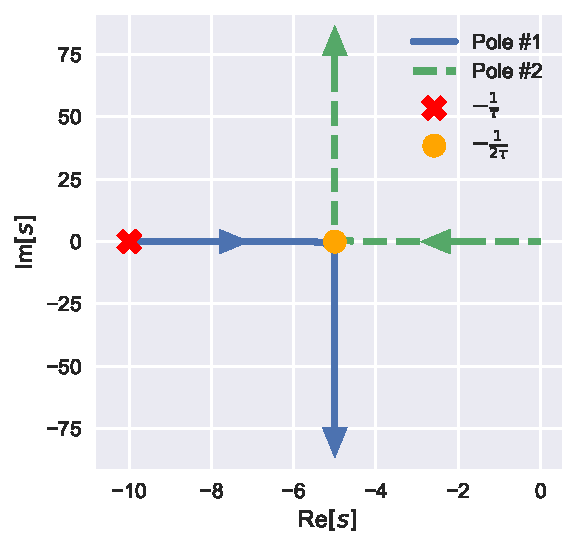
\includegraphics[width=0.4\textwidth]{pes-poles}
\caption{ \label{fig:pes-poles}
  Visualizing the poles of $F(s)$ (equation~\ref{eq:poles}) by sweeping $\kappa > 0$ (while $\| \V{a} \|^2$  and $\tau = 0.1\,$s remain fixed).
  Arrows follow the direction of \emph{increasing} $\kappa$.
  When $\phi \le \frac{1}{4}$, the dynamics of PES are a double-exponential.
  The learning rule becomes an alpha filter when the two poles collide: $\phi = \frac{1}{4} \iff s = -\frac{1}{2\tau}$ (marked by a solid circle).
  When $\phi > \frac{1}{4}$, the weight changes become oscillatory (due to complex poles).
  As $\kappa$ increases, the oscillatory frequency, $\omega$, scales as $\mathcal{O}\left(\sqrt{\kappa}\right)$.
  As $\kappa$ decreases, the first pole converges to $s = -\frac{1}{\tau}$ (marked by a solid \texttt{x}) while the second pole cancels the zero at $s = 0$. %(i.e.,~$F(s) = -H(s)$, $s \ne 0$).
  Reproduced from \citet[][Figure~4]{voelker2017c}.
}
\end{figure}

\subsection{Optimization}

There is extensive literature on the general topic of implementing optimization algorithms in the form of dynamical systems, dating back at least to the work of \citet{brockett1991dynamical}.
% But we are not aware of any reviews at this level where we are concerned with implementation details into consideration.
\citet{voelkerimplementing} noticed that the ``hill climbing'' algorithm may be cast as a dynamical system, and leveraged this to construct an SNN that locally searches across an error landscape.
This observation naturally extends to any gradient-based algorithm, since these algorithms are expressed as state-vectors that update continuously according to some (possibly nonlinear) function of the state of the system. 
Instances of this include gradient descent, feedback alignment~\citep{stockel2019align}, Bayesian inference, and expectation-maximization~\citep{sharma2017}.

Apart from what has been done in the NEF, there exist many other dynamical systems that solve optimization problems, that could just as easily be realized using Principle 3, including:
compressed sensing~\citep{kim2007interior},
sparse coding~\citep[LASSO;][]{shapero2014optimal, tang2017sparse},
dictionary learning~\citep{lin2018dictionary},
Hopfield networks~\citep{hopfield1982, frady2019robust},
non-negative similarity matching~\citep{pehlevan2019spiking},
and various other algorithms related to eigenvalues,
% principle component analysis,
independent component analysis,
and non-negative matrix factorization.
But rather than focusing on any one of these algorithms in particular, we turn our efforts to developing a comprehensive understanding of how the NEF may be extended to implement all of them.
